%   *******************************************************************
%   * THIS IS THE MAIN FILE--RUNNING LATEX ON "main.tex" WILL  *
%   * GENERATE THE ENTIRE THESIS (ASSUMING YOU HAVE NOT RENAMED IT).  *
%   * IF YOU ARE USING BIBTEX, RUNNING BIBTEX ON "AllegThesis" SHOULD *
%   * GENERATE YOUR BIBLIOGRAPHY. SPECIFIC DETAILS DEPEND ON WHAT     *
%   * ENVIRONMENT AND TOOLS YOU ARE USING (E.G., TEXMAKER OR COMMAND  *
%   * LINE TOOLS LIKE PDFLATEX OR ...).                               *
%   *******************************************************************
%
% main.tex
% by A. Thall
% 13 Feb 2003
%
% Revised by R. Roos
% Nov 2013
%
% This document provides a sample Senior Thesis template for use
% by students in Allegheny's CS and Applied Computing programs.
%
%   *******************************************************************
%   * LOOK FOR BLOCK COMMENTS SUCH AS THIS ONE FOR AN EXPLANATION OF  *
%   * THIS DOCUMENT AND HOW TO MODIFY IT FOR YOUR OWN THESIS!         *
%   *                                                                 *
%   * ANY LINE BEGINNING WITH A "%" IS A LATEX COMMENT AND IS IGNORED *
%   * BY THE LATEX PROCESSOR. YOU ARE ENCOURAGED TO COMMENT YOUR OWN  *
%   * LATEX CODE TO HELP YOU REMEMBER WHY YOU DID THINGS A CERTAIN WAY*
%   *******************************************************************
%

%   ********************************************************************
%   * THE FIRST SECTION OF THE MAIN LATEX FILE IS THE "PREAMBLE." IT   *
%   * INSTRUCTS LATEX TO IMPORT SPECIAL PACKAGES FOR THINGS LIKE       *
%   * INCLUDING FIGURES, DOUBLE-SPACING, COLORED TEXT, ETC.            *
%   * DEPENDING ON YOUR NEEDS, YOU MAY FIND IT NECESSARY TO USE PACK-  *
%   * AGES THAT ARE NOT INCLUDED IN THIS TEMPLATE. SIMPLY IMITATE THE  *
%   * "\usepackage{...}" COMMANDS SHOWN BELOW.                         *
%   ********************************************************************

%   ********************************************************************
%   * BEGINNING OF PREAMBLE:                                           *
%   ********************************************************************

\NeedsTeXFormat{LaTeX2e}
\documentclass[12pt]{report}

%   ********************************************************************
%   * ALL BUT ONE OF THE FOLLOWING 5 LINES SHOULD BE COMMENTED OUT.    *
%   * (NOT ALL OF THESE OPTIONS HAVE BEEN TESTED IN THIS REVISION!)    *
%   ********************************************************************

%\usepackage[debug,draft,double]{gatorthesis} % for student proof doublespace
%\usepackage[bottom,double]{gatorthesis} % for final department copy
\usepackage[debug,draft,single]{gatorthesis} % for student workcopy
%\usepackage[single]{gatorthesis} % for student
%\usepackage[debug,draft,nolists,nofront,single]{gatorthesis} % more options

% %% -- Typesetting -----------------------------------------------------
\usepackage[utf8]{inputenc}
\usepackage[english]{babel}
\usepackage[T1]{fontenc}
\usepackage{booktabs}
\usepackage{lmodern}
\usepackage{comment}     % provides a way to "comment out" sections in blocks
\usepackage{doublespace} % final document should be double-spaced!
\usepackage{enumitem}

% %% -- Listings  & Pseudocode ------------------------------------------
\usepackage[chapter]{minted}
\setminted{ fontfamily=lmtt
          , style=trac
          , mathescape = true
          }
\newminted[inlinerust]{rust}{ frame = leftline
                            , framerule = 0.4pt
                            , framesep = 2mm
                            , linenos = true
                            , numberblanklines = true
                            }
\newminted[inlinelisp]{lisp}{ frame = leftline
                            , framerule = 0.4pt
                            , framesep = 2mm
                            , linenos = true
                            , numberblanklines = true
                            }
\newmintedfile[apprust]{rust}{ fontsize=\footnotesize
                             , linenos = true
                             , numberblanklines = true
                             }
\usepackage{fancyvrb}
\usepackage[nounderscore]{syntax}
\def\<#1>{\synt{#1}} % allows `\<name>` to be used for nonterminal symbols
\usepackage{placeins}
\usepackage[figure]{algorithm2e}

%% -- Math ------------------------------------------------------------
\usepackage{amsmath,amssymb}
\usepackage{mathptmx}

%% -- Referencing -------------------------------------------------------
\usepackage{hyperref}
\usepackage{cleveref}
\usepackage[ backend=bibtex
           , style=numeric
           , sortcites=true
           , sorting=nty
           , backref
           , natbib
           , hyperref
           ]{biblatex}
\bibliography{bibliography/thesis.bib}


%% -- Figures ----------------------------------------------------------
\usepackage{epsfig}      % needed for including figures
% \usepackage{fancybox}  % --- DISABLED BY RSR, SEP 2013 ---
\usepackage{graphicx}

\usepackage{url}

% -- Definitions ------------------------------------------------------
\usepackage[framed,amsthm,hyperref]{ntheorem}

\theoremstyle{break}
\theoremheaderfont{\bf}\theorembodyfont{\itshape}

\theorempreskip{\topsep}
\theorempostskip{\topsep}
\theoremseparator{:}
\newtheorem{defn}{Definition}

%   ********************************************************************
%   * OPTIONAL: IF YOU WANT VERY FINE CONTROL OVER HOW LATEX HYPHENATES*
%   * CERTAIN WORDS, YOU CAN PUT WORDS IN A "\hyphenation" COMMAND AS  *
%   * SHOWN IN THE FOLLOWING EXAMPLE. OTHERWISE, YOU MAY JUST IGNORE   *
%   * THE NEXT COMMAND.                                                *
%   ********************************************************************

% EXAMPLE: Don't hyphenate the words "itself" or "linear". Hyphenate
%          "representations" only at the places indicated by the "-":

\hyphenation{itself repre-sen-tations linear}

%   ********************************************************************
%   * THE FOLLOWING COMMAND HAS BEEN DISABLED--IGNORE.                 *
%   ********************************************************************
% The following provides a box to surround the thesis statement
%\newenvironment{Thesis}%
%{\begin{Sbox}\begin{minipage}{.95\linewidth}}%
%{\end{minipage}\end{Sbox}\begin{center}\fbox{\TheSbox}\end{center}}

%   ********************************************************************
%   ********************************************************************
%   ***  END OF PREAMBLE.                                            ***
%   ********************************************************************
%   ********************************************************************



%   ********************************************************************
%   * DOCUMENT CONTENT STARTS AT THE "\begin{document}" COMMAND:       *
%   ********************************************************************

\begin{document}

%   ********************************************************************
%   * FILL IN THE "{...}" BELOW WITH YOUR INFORMATION.                 *
%   ********************************************************************

\thesistitle{Mnemosyne: A Functional Systems~Programming Language}

\thesisauthor{Hawk Weisman} \thesisadvisor{Dr. Robert Roos}

\thesisnumber{CS2016-12}

\thesisreadera{John Wenskovitch}


%   ********************************************************************
%   * IN RARE CASES YOU MAY HAVE MORE THAN TWO READERS, IN WHICH CASE  *
%   * YOU SHOULD UN-COMMENT THE FOLLOWING AND ADD NAMES:               *
%   ********************************************************************
% \thesisreaderb{Dr. Your Thirdreader}
% \thesisreaderc{Dr. Your Fourthreader}
% \thesisreaderd{Dr. Your Fifthreader}

%   ********************************************************************
%   * YOU MAY IGNORE THE FOLLOWING COMMAND:                            *
%   ********************************************************************
\date{\FileRevised \\ $\mbox{}$Revision: 1.8 $\mbox{}$}

\thesismaketitle         % Creates the title page
\thesismakecopyright     % Creates the copyright page

%   ********************************************************************
%   * YOU MAY SPLIT YOUR THESIS INTO SEVERAL FILES AND "\include" THEM *
%   * AS SHOWN BELOW. FOR INSTANCE, FILE "abstract.tex" CONTAINS THE   *
%   * ABSTRACT, FILE "ack.tex" CONTAINS THE ACKNOWLEDGMENTS, ETC. YOU  *
%   * MAY, OF COURSE, PUT EVERYTHING INTO ONE HUGE FILE, BUT THERE ARE *
%   * ADVANTAGES TO SPLITTING THINGS UP--FOR EXAMPLE, YOU CAN COMMENT  *
%   * OUT "\include" LINES OF SOME PARTS IN ORDER TO PRINT DRAFTS      *
%   * CONTAINING SELECTED SECTIONS OF YOUR THESIS, SAVING PAPER AND    *
%   * PRINTING COSTS.                                                  *
%   *                                                                  *
%   * YOU ARE NOT REQUIRED TO HAVE A "dedication"--IF YOU DON'T, JUST  *
%   * DELETE THAT LINE OR COMMENT IT OUT WITH A LEADING "%"            *
%   ********************************************************************

\begin{abstract}
Using \LaTeX\ to produce a professional-looking senior thesis can
be a daunting task. This work illustrates some of the more common
tools and features of \LaTeX. The PDF version of the thesis, together with
the heavily-commented {\tt .tex} source files used to produce it,
answer many questions commonly asked by
seniors concerning the final typeset thesis document.
\end{abstract}
  % REQUIRED!

\include{dedication} % OPTIONAL

\include{ack}       % OPTIONAL, BUT ALMOST EVERYONE INCLUDES IT

%   ********************************************************************
%   * FRONT MATTER--TABLE OF CONTENTS, ETC. YOU PROBABLY DON'T NEED TO *
%   * CHANGE ANY OF THIS UNLESS YOU HAVE NO TABLES OR FIGURES, OR YOU  *
%   * WANT TO CHANGE NUMBERING DEPTH FOR SUBSECTIONS, OR ...           *
%   ********************************************************************

\setcounter{tocdepth}{2}    % # of section levels shown in table of contents
\setcounter{secnumdepth}{3} % # of numbered subsection levels in the text

\tableofcontents
%\listoftables       % OMIT THIS IF YOU DON'T HAVE ANY TABLES
\listoffigures      % OMIT THIS IF YOU DON'T HAVE ANY FIGURES
\listoflistings


%   ********************************************************************
%   * A GLOSSARY IS ALMOST NEVER NEEDED UNLESS YOU HAVE AN UNUSUALLY   *
%   * LARGE NUMBER OF SPECIAL TERMS OR NOTATIONS AND IT WOULD DETRACT  *
%   * TOO MUCH FROM THE FLOW OF THE PAPER TO DEFINE THEM IN-LINE.      *
%   ********************************************************************
%\include{glossary}  % OMIT THIS IF YOU DON'T HAVE A GLOSSARY (FEW PEOPLE DO)


%   ********************************************************************
%   * THE FOLLOWING "lstset" COMMAND IS ADAPTED FROM ONE FOUND AT:     *
%   * http://tex.stackexchange.com/questions/115467/                   *
%   * listings-highlight-java-annotations                              *
%   *                                                                  *
%   * SEE CHAPTER 3 AND APPENDIX A                                     *
%   ********************************************************************

% I've disabled the "lstset" command since I'm using minted to prepare
% listings, instead. -- Hawk

% \lstset{          %  --- DISABLED BY MHW, NOV 2015 ---
%   basicstyle=\footnotesize\tt, % the size of the fonts that are used for the code
%   breakatwhitespace=false,     % automatic breaks only happen at whitespace?
%   breaklines=true,             % sets automatic line breaking
%   captionpos=b,                % sets the caption-position to bottom
%   frame=single,                % adds a frame around the code
%   language=Java,               % the language of the code
%   keywordstyle=\bf,
%   showspaces=false,
%   showstringspaces=false,      % underline spaces within strings only?
%   showtabs=false,
%   tabsize=2                    % sets default tabsize to 2 spaces
% }

%   ********************************************************************
%   * NOW INCLUDE THE CHAPTER FILES; COMMENT OUT ANY YOU DON'T WANT TO *
%   * PROCESS IN A PARTICULAR LATEX RUN.                               *
%   *                                                                  *
%   * INCLUDED FILES ARE ASSUMED TO END IN ".tex", E.G.,               *
%   * "ch01_overview.tex", "ch02_relatedwork.tex", ETC.                *
%   ********************************************************************

% ch:intro
%
% $Id: ch01_overview
%
%   *******************************************************************
%   * SEE THE MAIN FILE "AllegThesis.tex" FOR MORE INFORMATION.       *
%   *******************************************************************

\chapter{Introduction}\label{ch:intro} % we can refer to chapter by the label

\epigraph{ For last year's words belong to last year's language \\
           And next year's words await another voice. }%
         { \textit{Four Quartets} \\ \textsc{T.S. Eliot} }

The design and implementation of programming languages has been a major area of study for most of the history of computer science as a discipline. Since only a small fraction of software is implemented in assembly language, it seems reasonable to surmise that the quality of programming languages has a major impact on the quality of software in general. While many have observed that a great programmer can write good code even in a bad language\footnote{And inversely, that a terrible programmer can write bad code even in a good language}, we should note that individuals with such wizardly skill\footnote{Or frightening incompetence} likely fall far outside of the bell curve distribution of programmer ability. For a majority of software developers, programming languages likely have at least some impact on software quality.

Given this observation, the programming languages community has, in recent years, produced a number of new programming languages, such as Haskell~\cite{jones2003haskell,hudak1992report}, Scala~\cite{odersky2004scala,odersky2004overview}, and others. These languages boast a number of qualities that support the fast and easy implementation of high-quality software, such as more expressive syntax and typing disciplines that uncover errors at compile-time. However, while the developers of application software have benefited significantly from recent advances in programming languages, the languages used in systems programming have changed little since the 1970s.

\begin{defn}[Systems Programming]
The branch of programming concerned with the implementation of operating systems, utilities, and libraries that provides services to other software rather than to a human user~\cite{Narten:2003:SP:1074100.1074850}.
\end{defn}

\textit{Systems programming} refers to the implementation of operating systems, device drivers, programming language standard libraries and runtime systems, and other types of software that provide services to other software rather than to the user~\cite{Narten:2003:SP:1074100.1074850,Shapiro:2006:PLC:1215995.1216004}. This is in contrast to \textit{application programming}, which is concerned with the implementation of application software, software with which the user interacts with directly or uses to accomplish a task or activity.

\section{Current State of the Art}\label{sec:stateofart}

The \textit{lingua franca} of systems programming is the C programming language~\cite{kernighan1988c}, which first appeared in 1972. While there have been revisions to the C standard in recent years~\cite{C11,C99} and new C compilers, such as \texttt{clang}~\cite{lattner2008llvm}, have been developed, C has changed very little since its creation. C is plagued by safety issues and can be very difficult to program in, especially for novice programmers or those unfamiliar with its challenges~\cite{Shapiro:2006:PLC:1215995.1216004,Ray:2014:LSS:2635868.2635922,Bhattacharya:2011:APL:1985793.1985817}.

Why, then, do systems programmers, who work in an area where safety and correctness is often vital, use such an old and difficult language almost exclusively? There are a number of reasons behind the systems programmer's hesitation to try more modern languages. Despite the rapid, ongoing increase in the capabilities of computing hardware, performance and efficiency in both time and space are still deeply important in systems code, as small drops in performance can have major impacts on the application software that relies on a system program~\cite{Shapiro:2006:PLC:1215995.1216004}. Applications programmers can often benefit from the use of slightly less efficient abstractions and structures if they compose well and are easily understood, but systems programmers have no such luxury.

Many modern programming languages exhibit characteristics not suitable for systems programming. Many require a heavyweight runtime environment, running in a virtual machine or interpreter, making them insufficiently ``close to the machine''. They may provide abstractions and semantics that are convenient for the programmer but which make the low-level control necessary for many systems tasks impossible. When faced with the tradeoff between programmer convenience and low-level access to the computer's hardware, the designers of these languages tend, not unreasonably, to choose the latter. While this choice has benefitted the implementors of computer applications greatly, it has also left systems programmers stuck with the relics of computing's past.

A particularly major issue, discussed in greater detail in ~\Cref{sec:gc}, is that a vast majority of these languages manage memory automatically through garbage collection~\cite{Bartley:2003:GC:1074100.1074419,Dijkstra:1978:OGC:359642.359655}. While garbage collection means that programmers no longer have to worry about managing memory allocation and deallocation, it also means that this work must be performed at runtime. This interrupts the program's execution –– often unsuitable for systems software -- and requires runtime support from the garbage collection software~\cite{Bartley:2003:GC:1074100.1074419,Hertz:2005:QPG:1094811.1094836,Dijkstra:1978:OGC:359642.359655}.

%
% %   ************************************************************************
% %   * In LaTeX, new paragraphs are begun by simply leaving a blank line in *
% %   * the LaTeX file.                                                      *
% %   *                                                                      *
% %   * The \\ characters should NEVER be used to end a paragraph.           *
% %   * They are used only for inserting line breaks in certain situations.  *
% %   *                                                                      *
% %   * "Widows" (ending paragraph lines at the top of a new page) and       *
% %   * "orphans" (opening paragraph lines at the bottom of a page) should   *
% %   * be eliminated; this sometimes requires re-writing some of the        *
% %   * text to change the line lengths.                                     *
% %   ************************************************************************
%
% The purpose of this sample thesis is to show various \LaTeX\ formatting
% commands. Information about content should be obtained through consultation
% with the thesis readers and examination of past senior theses.
% There are no fixed rules governing the number of chapters or their titles---old
% senior theses and discussions with the thesis readers are the best resources
% for making such decisions.
%
% Usually, a chapter begins with a paragraph or two that serves as a
% sort of mini-introduction to the chapter. This is followed
% by numbered sections created with ``\verb$\section{...}$'',
% ``\verb$\subsection{...}$'', etc.
%
% \section{Motivation} \label{sec:motivation}
% The first paragraph in each section is not indented---that is a standard style
% that is enforced by the \LaTeX\ program. It should never be necessary to
% insert commands to force paragraph indentation.
%
% The thesis should avoid the use of second-person pronouns such as ``you''
% and ``your,'' as well as the use of imperative statements (implied
% second-person) such as ``Look
% at \ldots'' or ``Consider the following example \ldots''.
% First person (``I,'' ``my,'' etc.) is sometimes acceptable,
% but should be used sparingly. (This is an appropriate topic
% for discussion with the first reader of the project.) Contractions (``don't'',
% ``can't'', etc.) are considered informal and should be avoided. Common
% abbreviations such as ``math'' for ``mathematics'' or ``comp'' for
% ``senior comprehensive project''  are also informal and not appropriate
% in the final thesis.
%
% Figures illustrating complex or hard-to-describe concepts are essential.
% All figures should be fully explained in the text. For example,
% Figure \ref{latexprocess} shows the first step in processing a senior thesis.
% The user files consist of the main file, {\tt AllegThesis.tex}, and zero or
% more additional files ({\tt ch01.tex}, {\tt ch02.tex} in the figure). Not shown
% in the figure are image files, the bibliography, and other included
% components (the ``\ldots etc.\ldots'' on the left side of the figure).
% Typing the command {\tt pdflatex} with the main file name
% produces a number of additional files, including an {\tt .aux} file (with
% information such a label references and citations),
% a table of contents, or {\tt .toc}, file, a printable {\tt .pdf} file, and
% a number of others, depending on the document.
%
% %   *******************************************************************
% %   * FIGURES ARE PLACED ACCORDING TO A SET OF CONSTRAINTS THAT CAN   *
% %   * BE MANIPULATED TO SOME DEGREE.                                  *
% %   * A SEARCH FOR "controlling latex floats" TURNS UP A NUMBER OF    *
% %   * SITES THAT HAVE USEFUL INFORMATION, FOR EXAMPLE:                *
% %   *                                                                 *
% %   * http://mintaka.sdsu.edu/GF/bibliog/latex/floats.html            *
% %   * http://goo.gl/aC8E8Q                                            *
% %   * http://robjhyndman.com/hyndsight/latex-floats/                  *
% %   *******************************************************************
%
% % \begin{figure}[htbp]
% % \centering
% % 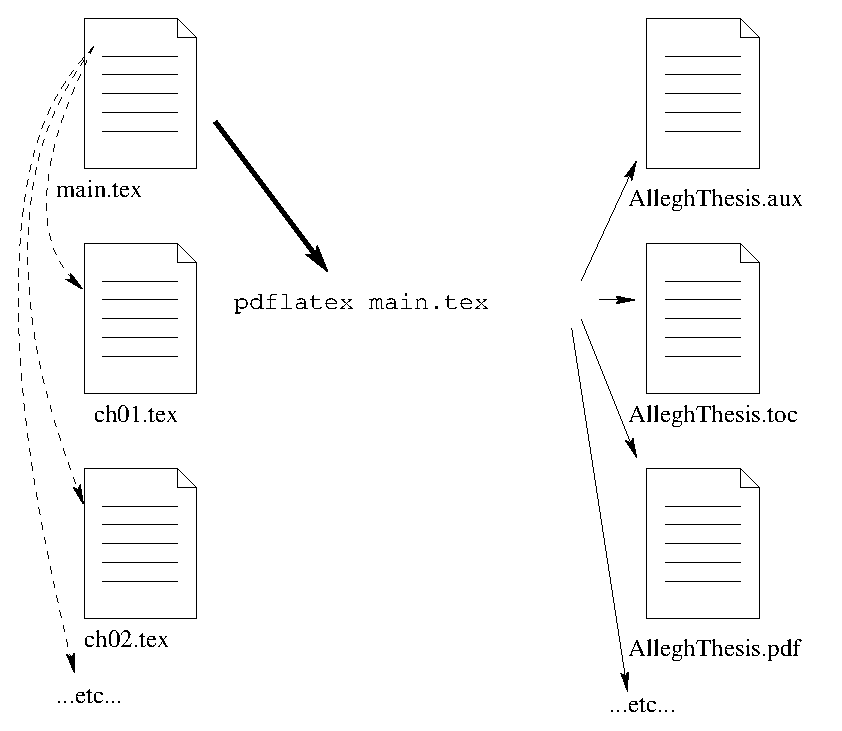
\includegraphics[width=3.5in]{latexprocess}
% % \caption{The first step in creating a thesis document}
% % \label{latexprocess}
% % \end{figure}
%
% \section{Current State of the Art}\label{sec:stateofart}
% There are multiple
% ways to create {\it italicized}, {\bf bold-face}, {\tt fixed-width}, and
% {\sf sans-serif} fonts, as well as combinations, e.g., \textit{\textbf{
% bold italic}} or \textit{\textsf{italic sans-serif}}. The \LaTeX\ source
% file for this chapter shows some of the ways to achieve these effects.
% It is customary to use fixed-width font for program constructs, e.g.,
% ``In the Java code accompanying the figure, {\tt n} stands for the
% number of generations to be simulated by the {\tt evolvePopulation()} method.''
% Variables in mathematical equations are normally rendered in
% italics, e.g., ``In the performance equation, {\it cpuTime} is
% the average time over fifty runs of the program.''
%
% %It is the privilege of the thesis author (in consultation with the
% %project supervisor and other readers) to decide on the best way to
% %organize the sections and chapters in the way that makes the most sense.
% %If the introduction begins with a motivating
% %anecdote, perhaps this is best followed by defining a few terms or mentioning
% %some major results that the reader should be aware of right from the
% %beginning. But
% It is important to get as quickly as possible to
% a concise statement of the {\it thesis}---the main question
% addressed by the project. This might merit a separate
% section of the chapter.
%
\section{Goals of the Project}\label{sec:goals}
% This section could also be entitled ``Thesis'' or something similar.
% A formal thesis statement should be a
% %\emph{falsifiable} % COMMENT OUT THINGS THAT YOU MAY LATER WISH TO PUT BACK
% statement about
% the goal achieved by the project.  For a purely scientific
% project, this is the hypothesis being tested; it should be a
% \emph{falsifiable} statement, i.e., one that can be disproven through
% an appropriate experiment.
% For an applied programming project, it is usually a statement about
% the feasibility and correctness of the approach used and the advantages it
% has over other approaches, using suitable metrics.  For a survey or study,
% it is usually a statement regarding the need
% or usefulness of such a study, its intended audience, and so on.
% % COMMENTED OUT NEXT FEW LINES TO SAVE SPACE; MAY PUT THEM BACK LATER
% %Following the concise statement of the thesis, some of the details can be
% %expanded.
% %It is appropriate to
% %refer to some of the results in the introduction (which may
% %mean going back and adding them to the introduction once the
% %research is completed).
% %A senior thesis, or any research paper, is not a mystery
% %novel---there is no need to keep the reader in suspense about what
% %has been accomplished.

Mnemosyne\footnote{Named for the Titaness who personified the concept of memory in Greek myth.} is a new programming language intended for systems programming. Mnemosyne is intended to reconcile the requirements of low-level systems implementation with the safety, expressive power, and elegance of modern functional programming languages.

\section{Thesis Outline}\label{sec:outline}

\Cref{ch:background} provides greater detail into the rationale behind Mnemosyne's creation and reviews preceding work in the area. \Cref{ch:design} discusses the considerations involved in the design of Mnemosyne's syntax and semantics, while \Cref{ch:implem} describes the implementation process for the prototype Mnemosyne compiler. In \Cref{ch:eval}, methods of evaluating the correctness of the Mnemosyne compiler prototype are discussed, and the results of these evalautions analyzed. Finally, \Cref{ch:conclusion} concludes this thesis with a summation of the outcomes of the research and a discussion of potential avenues for future work.
 % Introduction -- of course, you can name it anything!

% ch:relatedwork
%
% $Id: ch02_background
%
%   *******************************************************************
%   * SEE THE MAIN FILE "AllegThesis.tex" FOR MORE INFORMATION.       *
%   *******************************************************************
\chapter{Background and Rationale}\label{ch:relatedwork}

\epigraph{ If I have seen further, it is by standing
           on the shoulders of giants. }%
         { Letter to Robert Hooke, February 5, 1676 \\
           \textsc{Sir Isaac Newton} }

% A typical second chapter deals with a survey of the literature
% related to the thesis topic. The subsections may be organized in whatever
% manner seems best suited to the material---chronological, or by topic, or
% according to some other criteria (e.g., primary versus secondary resources).
% The examples given in the sections in this chapter are nonsensical in content;
% they are provided merely to give examples of citing bibliographic references.
% Resources should be cited by author name(s), not by title.
% There should be a space between the square brackets of a citation and
% any preceding words. Thus, ``Smith and Jones[17]'' is wrong; ``Smith and
% Jones [17]'' is correct. If the citation is at the end of a sentence, the
% period goes after the brackets (``Johnson [23].'', not ``Johnson. [23]'').
%
% \section{Primary Sources}
% The earliest work done in widget software is described in the seminal 1986
% paper by Smith and Jones \cite{SmithJones86}. Using a networked array of
% high-performance computers they demonstrate that widgets with $k$ degrees
% of freedom can be simulated in time proportional to $k\log^2k$. At the
% heart of their demonstration is an algorithm for re-encabulating the widgets
% using a lookup table that can be updated in real time, assuming that
% the widgets are non-orthogonal. The question of simulating orthogonal widgets
% is left open, but the authors conjecture that orthogonality will add at
% most another factor of $k$ to the performance upper bound.
%
%
% \section{Recent Results}
% A number of papers \cite{blum67,damon:95,zobel:97} deal with issues
% that are peripheral to the orthogonal case, but Dio\c{s}an and Oltean
% were the first to tackle it directly.
% In their 2009 paper \cite{diosan09},
% Dio\c{s}an and Oltean apply evolutionary techniques to
% the orthogonal widget case, obtaining empirical results that suggest
% an efficient algorithm might be at hand. Their
% approach is characterized by the use of a genetic algorithm to evolve other,
% more problem-specific evolutionary algorithms.
 % Background, literature survey, ...

% ch:design
%
% $Id: ch03_design.tex
%
%   *******************************************************************
%   * SEE THE MAIN FILE "main.tex" FOR MORE INFORMATION.       *
%   *******************************************************************
%
\chapter{Design Considerations} \label{ch:design}

\section{Design Goals} \label{sec:goals}

The following characteristics are major design goals for Mnemosyne:
\begin{enumerate}
    \item Support for systems programming
    \item Safety
    \item Performance
    \item Support for quality programming
    \item Expressiveness
\end{enumerate}

\paragraph{Expressiveness}
%
% Formally, the \textit{expressiveness} (or \textit{expressive power}) refers to the size of the set of all ideas or concepts capable of being communicated by a language. As a general-purpose programming language, Mnemosyne is intended to be Turing-complete; meaning that theoretically, all possible computations can be expressed in Mnemosyne. In the context of general-purpose, Turing-complete languages, this term is more foten used to refer to the

\section{Characteristics} \label{sec:characteristics}

Programming languages may be categorized along a number of axes: whether it is compiled or interpreted, its typing discipline, what programming paradigms it is inteded to support, its method of memory management, and others.

Mnemosyne is a \textit{statically-typed} programming language, meaning that the analysis of the types of language constructs, such as variables and expressions, are known to the compiler at compile-time. This is in contrast to \textit{dynamically-typed} languages, such as a majority of the Lisp family, in which types are determined at runtime.

A major advantage of static typing lies in its increased reliability. If we suppose that some operations are not supported on all types, and that attempting these operations on types which are not capable of carrying them out results in an error, as is the case in almost all programming languages, then such \textit{type errors} are a cadegory of potential error which may occur in our programs. In a statically-typed language, the compiler has the capacity to reason about types, and thus these type errors can be detected at compile-time; while in a dynamically typed language, type errors will occur during the program's execution. Moving the detection of an entire category of errors from runtime to compile-time is a major boon to the language's reliability and safety.

% Furthermore, many programming languages use their type systems to encode other potential categories of errors in their type systems. If, for example, we encode some property such as the lengths of arrays at the type level,

Additionally, giving the compiler the capacity to reason about types permits us to perform a number of optimizations that are not possible in dynamically-typed languages.
% \section{Test Environment}
% Algorithm \ref{widgmin} (from \cite{Fiori:2013}) shows a high-level description of an
% algorithm. There are many options for the display of
% pseudocode; this uses the {\tt algorithm2e} package \cite{Fiori:2013},
% but there are a number of others available at the Comprehensive \TeX\ Archive
% Network (\url{ctan.org}). Using any of these
% other packages might require the additon of one or more
% ``\verb$\usepackage{...}$'' commands in the main {\tt main.tex} file.

%   *******************************************************************
%   * SEE CHAPTER ch_01overview.tex FOR INFORMATION ON CONTROLLING    *
%   * PLACEMENT OF FIGURES.                                           *
%   *                                                                 *
%   * THERE ARE MANY DIFFERENT ALGORITHM ENVIRONMENTS. HERE, WE USE   *
%   * THE "algorithm2e" PACKAGE, BUT YOU SHOULD LOOK TO SEE IF        *
%   * OTHER PACKAGES BETTER MEET YOUR NEEDS. REGARDLESS OF WHICH      *
%   * PACKAGE YOU USE, EXPECT TO SPEND TIME READING THE USER MANUAL   *
%   * AS THERE ARE USUALLY A LARGE NUMBER OF PARAMETERS THAT CAN      *
%   * SIGNIFICANTLY AFFECT THE FINAL APPEARANCE OF THE ALGORITHM.     *
%   *******************************************************************
%
% \begin{algorithm}[htbp]
%  %\SetLine % For v3.9
%  \SetAlgoLined % For previous releases [?]
%  \KwData{this text}
%  \KwResult{how to write algorithm with \LaTeX2e }
%  initialization\;
%  \While{not at end of this document}{
%   read current\;
%   \eIf{understand}{
%    go to next section\;
%    current section becomes this one\;
%    }{
%    go back to the beginning of current section\;
%   }
%  }
%  \caption{How to write algorithms (from \cite{Fiori:2013})}
% \label{widgmin}
% \end{algorithm}

\section{Experiments}

% Figure \ref{javaprog} shows a Java program. There are many, many options for
% providing program listings; only a few of the basic ones are shown
% in the figure. Some thought must be given to making code suitable
% for display in a paper. In particular long lines, tabbed indents, and
% several other practices should be avoided. Figure \ref{javaprog} makes
% use of the {\tt listings} style file \cite{Heinz:2013}.

%   *******************************************************************
%   * SEE CHAPTER ch_01overview.tex FOR INFORMATION ON CONTROLLING    *
%   * PLACEMENT OF FIGURES.                                           *
%   *                                                                 *
%   * SEE THE MAIN FILE "main.tex" FOR THE "\lstset" COMMAND   *
%   * THAT DEFINES HOW PROGRAM LISTINGS WILL LOOK.                    *
%   *                                                                 *
%   * AS WITH EVERYTHING IN LATEX, LOOK AT THE USER MANUAL, SEARCH    *
%   * FOR EXAMPLES ONLINE, CUSTOMIZE TO GET A PLEASING LOOK.          *
%   *******************************************************************


% \begin{figure}[htbp]
% \centering
% \lstinputlisting{SampleProgUncommented.java}
% \caption{{\tt SampleProg}: A very simple program}
% \label{javaprog}
% \end{figure}

\section{Threats to Validity}
 % Chapter organization is topic-dependent

%ch:implem
%
% $Id: ch04_implementation.tex
%
%   *******************************************************************
%   * SEE THE MAIN FILE "AllegThesis.tex" FOR MORE INFORMATION.       *
%   *******************************************************************
%
\chapter{Implementation}\label{ch:implem}
The Mnemosyne compiler, called \texttt{mn}\footnote{Pronounced ``Manganese''.} operates in three primary phases:

\begin{itemize}
\item \textbf{Semantic analysis} converts the program source code to a representation understandable by the compiler and detects syntax errors
\item \textbf{Semantic analysis} attempts to prove statements about the program's execution, such as determining the types of values and reducing expressions to constants, and detects semantic errors
\item \textbf{Code generation} converts the internal representation of the program to LLVM intermediate representation (IR) and then to the desired output binary format.
\end{itemize}

\section{Parsing and Syntactic Analysis}\label{sec:parsing}
The Mnemosyne parser is implemented using technique called \textit{combinator parsing}.

\section{Semantic Analysis}\label{sec:analysis}
\section{Code Generation}\label{sec:codegen}
 % Chapter organization is topic-dependent

%ch:eval
%
% $Id: ch05_evaluation.tex
%
%   *******************************************************************
%   * SEE THE MAIN FILE "AllegThesis.tex" FOR MORE INFORMATION.       *
%   *******************************************************************
%
\chapter{Evaluation}\label{ch:eval}
Another possible chapter title: Experimental Results
 % Chapter organization is topic-dependent

%ch:conclusion
%
% $Id: conclusion.tex
%
%   *******************************************************************
%   * SEE THE MAIN FILE "AllegThesis.tex" FOR MORE INFORMATION.       *
%   *******************************************************************
%

\chapter{Discussion and Future Work}\label{ch:conclusion}
\epigraph{ The future will be better tomorrow. }
         { \textsc{Dan Quayle} }

This chapter usually contains the following items, although not
necessarily in this order or sectioned this way in particular.

\section{Summary of Results}
A discussion of the significance of the results
and a review of claims and contributions.

\section{Future Work}

\section{Conclusion}
 % Conclusion/future work

%   ********************************************************************
%   * IF YOU HAVE ANY APPENDICES (FOR INSTANCE, CODE, DATA, GRAPHS,    *
%   * OR ANYTHING ELSE THAT DOESN'T "FIT" AS REGULAR CHAPTER CONTENT), *
%   * INCLUDE THE FOLLOWING LINE, WHICH INSTRUCTS LATEX TO CHANGE FROM *
%   * NUMBERED "CHAPTER" HEADINGS TO LETTERED "APPENDIX" HEADINGS.     *
%   *                                                                  *
%   * APPENDICES HAVE THE SAME FORMATTING COMMANDS AS CHAPTERS (E.G.,  *
%   * "\chapter{...}", "\section{...}", ETC.)                          *
%   ********************************************************************

\appendix
 % Appendices go here

%app:spec
% Appendix A: Mnemosyne Grammar
% $Id: app-spec
%
%   *******************************************************************
%   * SEE THE MAIN FILE "main.tex" FOR MORE INFORMATION.       *
%   *******************************************************************

\chapter{The Mnemosyne Programming Language: An Abridged Description}\label{app:spec}
\setlength{\grammarindent}{6em}

The following is an abbreviated description of the Mnemosyne programming language. It is for illustrative purposes only and is not intended as a complete formal specification.

Please note that as the Mnemosyne compiler is currently an early prototype, it may not behave exactly as described in this document. While the compiler remains in the prototype stage (i.e., prior to the release of version 1.0.0), please regard this document as the only description of the canonical behaviour of a standards-compliant Mnemosyne compiler.

\subsection{Syntactic Notation}
Syntax descriptions are written using an extended BNF notation, as follows:
\begin{description}[leftmargin=3cm,labelindent=\parindent]
    \item{\synt{symbol}} indicates a non-terminal symbol
    \item{\lit{symbol}} indicates a terminal symbol
    \item{\synt{symbol}* } indicates zero or more repetitions of \synt{symbol}
    \item{\synt{symbol}+} indicates one or more repetitions of \synt{symbol}.
    \item{$\varepsilon$} indicates the empty string
\end{description}

The following special symbols refer to specific Unicode characters:
\begin{description}[leftmargin=3cm,labelindent=\parindent]
    \item{\synt{lambda}} Greek capital letter Lambda (U+03BB)
    \item{\synt{arrow}} Rightwards arrow (U+2192)
    \item{\synt{double arrow}} Rightwards double arrow (U+21D2)
    \item{\synt{tab}} Character tabulation (U+0009)
    \item{\synt{linefeed}} Linefeed (U+000A)
    \item{\synt{return}} Carriage return (U+000D)
    \item{\synt{space}} Space (U+0020)
\end{description}

Finally, the symbol \synt{any} refers to any character.

\section{Program Structure}

All Mnemosyne programs consist of one or more \textit{modules}. A module forms the top level of a Mnemosyne program and represents a namespace within which types and functions may be defined. A module then consists of a series of one or more \textit{definitions} (\Cref{sec:def}) and \textit{expressions} (\Cref{sec:expr}). An expression is a value-level construct: all expressions can be evaluated to some value, either at run-time or at compile-time. Definitions, by contrast, are type-level constructs.

\section{Lexical Syntax}\label{sec:lexical}
This section describes the lexical structure of Mnemosyne programs.

Mnemosyne uses the Unicode character set. While Mnemosyne programs written in the ASCII character set are considered valid, a standards-compiliant Mnemosyne compiler should be capable of recognizing Unicode characters. Unicode support is necessary both because certain non-alphanumeric Unicode characters not present in ASCII have defined meanings in Mnemosyne programs, and in order to ensure that Mnemosyne programs may be written in languages other than English. Note that Mnemosyne's lexical syntax then depends on the properties of the Unicode encoding as defined by the Unicode consortium. A standards-compilant Mnemosyne compiler should ensure compatiblity with new versions of the Unicode standard as they are released.

% \newcommand{\into}{$\longrightarrow$}
Note: \Cref{sec:code:parser} contains a source code listing for the Mnemosyne parser, and should be referred to to answer specific questions regarding how the reference Mnemosyne implementation handles specific characters.

% \begin{listing}[H]
    \begin{grammar}
        <program> $\to$ <token>+

        <token> $\to$ <lexeme> | <atmosphere>

        <lexeme> $\to$ <identifier> | <operator> | <keyword> | <literal>
                    \alt <sigil> | <delimiter>

        <sigil> $\to$ `@' | `&' | `*' | `\$' | `?'

        <delimiter> $\to$ `(' | `)' | `{' | `}'

        <identifier> $\to$ <initial> <subsequent>*

        <initial> $\to$ <letter> | <special initial>

        <subsequent> $\to$ <letter> | <number> | <special subsequent>

        <letter> $\to$ `a' | `b' | `c' | ... | `z'
                 \alt `A' | `B' | `C' | ... | `Z'

        <number> $\to$ `0' | `1' | ... | `9'

        <special initial> $\to$ `+' | `-' | `*' | `<' | `>' | `='
                          \alt `!' | `:' | `\%' | `^'

        <special subsequent> $\to$ <special initial> | `\'' | `_'

        <keyword> $\to$ `and' | `begin'  | `borrow' | `case' | `cond'
                  \alt `class' | `data' | `define' | `defn' | `def'
                  \alt `delay'| `do' | `else' | `if' | `instance'
                  \alt `impl' | `lambda' | `let' | `let*' | `letrec'
                  \alt `mod' | `or' | `quasiquote' | `quote' | `ref'
                  \alt `set!' | `struct' | `trait' | `type' | `typeclass'
                  \alt `union' |  `unquote' | `unquote-splicing'
                  \alt <lambda> | <arrow> | <fat arrow>
                  \alt <builtin type>
                  \alt \lit{|}  | `->' | `=>` | `,'

        <builtin type> $\to$ `i8' | `i16' | `i32' | `i64' | `int'
                        \alt `u8' | `ui6` | `u32' | `u64' | `uint'
                        \alt `f32' | `f64' | `float' | `double'
                        \alt `bool' | `string'

        <atmosphere> $\to$ <whitespace> | <comment>

        <whitespace> $\to$ <space>
                    \alt <tab> (U+0009)
                    \alt <linefeed> (U+000A)
                    \alt <carriage return> (U+000D)

        <comment> $\to$ `;' <any>* <line ending>
                  \alt \lit{\#|} <any>* \lit{|\#}

    \end{grammar}
    % \caption{Mnemosyne lexical syntax.}
% \end{listing}
\section{Expressions}\label{sec:expr}

Mnemosyne \textit{expressions} form the basic building block from which all Mnemosyne programs are constructed. An expression is defined as any sequence of Mnemosyne tokens which may be resolved to a value-level result, either by the compiler or during the execution of a program. This section describes the syntax and informal semantics of Mnemosyne expressions.

\begin{grammar}
    <expr> $\to$ <s-expr> | <i-expr> | <c-expr> | <n-expr>
            \alt <deref expr> | <unwrap expr> | <pointer expr>
            \alt <literal>

    <s-expr> $\to$ `(' <operator>  <expr>* `)'

    <c-expr> $\to$ `{' <expr> <operator> <c-expr body>+ `}'

    <c-expr body> $\to$ <expr> <operator>
                   \alt <expr>

    <n-expr> $\to$ <access> `(' <expr>* `)'
              \alt <access> `.' <identifier>
              \alt <access> `.' <n-expr>

    <access> $\to$ <deref-expr> | <identifier>

    <deref expr> $\to$ `(' \lit{\$} <expr> `)'
                  \alt \lit{\$} <expr>

    <unwrap expr> $\to$ `(' `?' <expr> <expr>`)'
                   \alt `(' `?' <expr> `)'
                   \alt `?'<expr>

    <pointer expr> $\to$ `(' <pointer sigil> <expr> `)'
                    \alt <pointer sigil> <expr>

    <pointer sigil> $\to$ `&' | `@' | `*'
\end{grammar}

\subsection{Program Structure}

\begin{grammar}
<program> $\to$ <module>+

<module> $\to$ <module-def> <definition>*

<module-def> $\to$ `(' `mod' <identifier> <exports-clause> `)'

<exports-clause> $\to$ `(' `exports' <identifier>+ `)'
                \alt $\varepsilon$


%% skip a bit
\end{grammar}

\section{Definitions}\label{sec:def}

\subsection{Attributes}\label{sub:attr}
% \begin{listing}
\begin{grammar}
<function-attrs> $\to$ \lit{\#(} <function-attr>* \lit{)}

<function-attr> $\to$ <any-attr>
                 \alt `cold'
                 \alt <inline>

<inline> $\to$ `inline'
          \alt `inline-always'

<data-attr> $\to$ <any-attr>
            \alt `(' `as' <as-attr>+ `)'
            \alt `as' `(' <as-attr>+ `)'

<as-attr> $\to$ `C' | `packed'
          \alt `u8' | `u16' | `u32' | `u64'
\end{grammar}
% \caption{Grammar for Mnemosyne attributes.}
% \end{listing}

%app:code
%
% $Id: appa--code
%
%   *******************************************************************
%   * SEE THE MAIN FILE "main.tex" FOR MORE INFORMATION.       *
%   *******************************************************************

\chapter{Manganese Source Code}\label{app:code}
All program code should be fully commented. Authorship
of all parts of the code should be clearly specified.

%   *******************************************************************
%   * SEE THE MAIN FILE "main.tex" FOR THE "\lstset" COMMAND   *
%   * THAT DEFINES HOW PROGRAM LISTINGS WILL LOOK.                    *
%   *******************************************************************

\section{Mnemosyne Core Crate}
% \begin{listing}[H]
    \paragraph{lib.rs}
    \apprust[label=Contents of the file \texttt{core/src/lib.rs}
            ]{appendices/source/core/src/lib.rs}
%     \caption{Contents of the file \texttt{core/src/lib.rs}}
%     \label{src:lib.rs}
% % \end{listing}
%
% \begin{listing}[H]
    \paragraph{chars.rs}
    \apprust{appendices/source/core/src/chars.rs}
%     \caption{Contents of the file \texttt{core/src/chars.rs}}
%     \label{src:chars.rs}
% \end{listing}
%
% \begin{listing}[H]
    \paragraph{errors.rs}
    \apprust{appendices/source/core/src/errors.rs}
%     \caption{Contents of the file \texttt{core/src/errors.rs}}
%     \label{src:errors.rs}
% \end{listing}
%
% \begin{listing}[H]
    \paragraph{forktable.rs}
    \apprust{appendices/source/core/src/forktable.rs}
%     \caption{Contents of the file \texttt{core/src/forktable.rs}}
%     \label{src:forktable.rs}
% \end{listing}
%
% \begin{listing}[H]
    \paragraph{position.rs}
    \apprust{appendices/source/core/src/position.rs}
%     \caption{Contents of the file \texttt{core/src/position.rs}}
%     \label{src:position.rs}
% \end{listing}
\
%
% \begin{listing}[H]
    \paragraph{compile/mod.rs}
    \apprust{appendices/source/core/src/compile/mod.rs}
%     \caption{Contents of the file \texttt{core/src/compile/mod.rs}}
%     \label{src:compile/mod.rs}
% \end{listing}


\section{Mnemosyne Parser Crate}
    % \label{sec:code:parser}%

    \paragraph{lib.rs}
    \apprust{appendices/source/parser/src/lib.rs}

    \paragraph{tests.rs}
    \apprust{appendices/source/parser/src/tests.rs}

\section{Manganese Application Crate}
    \paragraph{main.rs}
    \apprust{appendices/source/src/main.rs}%
    %


%   ********************************************************************
%   * THE FINAL COMMANDS DEAL WITH BIBLIOGRAPHY/REFERENCES. IF THERE   *
%   * ARE ANY ITEMS IN YOUR BIBTEX FILE THAT YOU DID NOT REFERENCE IN  *
%   * YOUR PAPER, BUT THAT YOU WISH TO INCLUDE IN THE BIBLIOGRAPHY,    *
%   * YOU MAY SPECIFY "\nocite" COMMANDS TO FORCE THEM TO BE INCLUDED. *
%   *                                                                  *
%   * THE COMMAND "\nocite{*}" FORCES EVERY ITEM IN YOUR BIBTEX FILE.  *
%   ********************************************************************

%\nocite{ckm-acmap-99}   % EXAMPLES OF FORCING THINGS TO BE INCLUDED
%\nocite{Dierckx93}      %   "   "   "
%\nocite{obs-stcav-92}   %   "   "   "
%\nocite{bb4471}         %   "   "   "

\nocite{*} % OR DO THIS TO INCLUDE ALL BIBTEX REFERENCES IN THE BIBLIOGRAPHY

% \bibliographystyle{plain}

%   ********************************************************************
%   * IF YOU HAVE YOUR BIBLIOGRAPHY IN A SEPARATE ".bib" FILE, HERE IS *
%   * WHERE YOU MUST SPECIFY IT. IN THIS EXAMPLE, THE BIBLIOGRAPHY     *
%   * ENTRIES ARE STORED IN A SUBDIRECTORY NAMED "Bibdir" IN A FILE    *
%   * NAMED "myBibtexDB.bib".                                          *
%   ********************************************************************

\begin{spacing}{1}
    \begingroup
    \setlength{\emergencystretch}{1em} % fixes overfull hboxes in citations
                                       % (according to the interwebs)
    \printbibliography
    \endgroup
\end{spacing}

%   ********************************************************************
%   * THIS FEATURE HAS BEEN DISABLED:                                  *
%   ********************************************************************
% \include{colophon}

\typeout{THEPAGE \thepage}

\end{document}
